Lo studio dell'articolo di Jerrum e Sinclair, l'analisi dei teoremi e dell'algoritmo derivante, la realizzazione dei miglioramenti nella stima della \textit{partition function} e del lavoro svolto sul \textit{mean magnetic moment} mostrati nei capitoli \ref{chap5} e \ref{chap6} sono sempre stati accompagnati da implementazione e testing. In tal modo si è potuto costruire in maniera incrementale, a partire da ciò che era già stato sviluppato in precedenza, analizzando accuratamente gli effetti delle scelte intraprese, decidendo di conseguenza sulla strada da percorrere.\\
Si descrive ora, nel dettaglio, come sono state realizzate le fasi di implementazione e testing.
\section{Implementazione}
Gli algoritmi proposti nei Capitoli \ref{chap5} e \ref{chap6} sono stati implementati utilizzando il linguaggio \textbf{Python}.
\paragraph{Python.} È un linguaggio di alto livello pubblicato nel 1991 dal suo autore \textit{Guido Van Rossum}: è general-purpose, interpretato, dinamico e largamente utilizzato. La sua filosofia di progettazione enfatizza la leggibilità del codice, e la sua sintassi permette ai programmatori di esprimere concetti in un minor numero di linee di codice rispetto ad altri linguaggi come \CC \space o Java. Il linguaggio fornisce costrutti pensati per produrre programmi su piccola e larga scala.\\
Python supporta molteplici paradigmi di programmazione, inclusa quella object-oriented, imperativa, funzionale e procedurale. È caratterizzato da un sistema di tipizzazione dinamico, dalla gestione automatica della memoria ed ha una libreria standard completa. Gli interpreti Python sono disponibili per i più diffusi sistemi operativi.
\begin{figure}[h!]
	\centering
	
\includegraphics[scale=.4]{img/Python_logo.png}
	\caption{Logo del linguaggio Python}
	\label{img:python}
\end{figure}
Il design di Python offre supporto alla programmazione funzionale nella tradizione Lisp. Il linguaggio è dotato delle funzioni \textit{map()} \textit{reduce()} e \textit{filter()}; \textit{list comprehension}, \textit{dizionari}, \textit{insiemi} e \textit{generators}.\\
La filosofia al cuore del linguaggio è riassunta dal documento ``\textit{The Zen of Python}'' (PEP 20), che include aforismi come:
\begin{itemize}
	\item \textit{Beautiful is better than ugly}
	\item \textit{Explicit is better than implicit}
	\item \textit{Simple is better than complex}
	\item \textit{Complex is better than complicated}
	\item \textit{Readability counts}
\end{itemize}
Un obiettivo importante degli sviluppatori Python è quello di rendere divertente il suo utilizzo, ciò è rispecchiato anche dal nome che deriva dai ``\textit{Monty Python}'', il celebre gruppo comico britannico, la cui commedia acutamente intellettuale riscosse grande successo tra gli anni '60 ed '80.
\subsection{Librerie utilizzate}
Se la potenza di un linguaggio di programmazione può essere misurata in librerie di cui dispone, allora Python è da considerarsi un linguaggio estremamente potente. Il \textit{Python Package Index} (PyPI), che è il più grande repository di software per il linguaggio Python, attualmente contiene 86483 pacchetti, ognuno dei quali liberamente scaricabile ed integrabile all'interno della propria applicazione, essendo rilasciato secondo una delle molteplici licenze Open Source.
\paragraph{NumPy.} È il pacchetto scientifico fondamentale per fare computazione scientifica in Python. Fornisce al linguaggio l'oggetto array multidimensionale, vari oggetti derivati (come array maschera e matrici) ed un vasto assortimento di routine per eseguire velocemente operazioni su array, incluse operazioni matematiche, logiche, manipolazioni di forma, ordinamenti, selezioni, I/O, trasformate di Fourier discrete, algebra lineare di base, operazioni statistiche di base, simulazioni casuali e molto altro. Maggiori dettagli alla pagina dedicata \cite{Numpy}.
\paragraph{joblib.} È un insieme di strumenti che forniscono supporto per il calcolo parallelo in Python. In particolare, joblib offre:
\begin{itemize}
	\item Caching su disco trasparente dei valori di output e lazy re-evaluation (pattern memoize)
	\item Semplici strumenti di supporto alla computazione parallela
	\item Logging e tracing dell'esecuzione
\end{itemize}
Joblib è ottimizzato per essere veloce e robusto, in particolare su molti dati ed ha specifiche ottimizzazioni per gli array numpy. Maggiori dettagli alla pagina dedicata \cite{joblib}.
\subsection{Strutture e librerie implementate}
\subsubsection{Strutture}
\paragraph{Grafo.} Il sistema di Ising ferromagnetico è rappresentato attraverso un grafo e costituisce l'input dell'algoritmo. Si è scelto di strutturare il grafo come una lista di triple, di cui ogni tripla rappresenta un arco: estremi dell'arco ed energia di interazione. Per ulteriori dettagli consultare \ref{sec:ising}.\\
Per convenienza, in alcuni casi, è stata anche utilizzata la classica rappresentazione in dizionario, le cui entry hanno come chiave il nodo ed i valori ad essa associati sono i suoi vicini.
\paragraph{Sottografo.} Un sottografo è rappresentato anch'esso come lista di triple, le cui tuple sono gli estremi del grafo ed un numero binario che indica se tale arco è presente nel sottografo in questione.
\subsubsection{Librerie}
Durante l'implementazione di questo lavoro di tesi, è stato necessario costruire delle librerie che offrissero supporto alla manipolazione di grafi e sottografi, oltre a varie procedure di generazione di grafi casuali ed iterazione di bitset ordinati.\\
Lo stile di scrittura del codice implementato rispecchia le linee guida del linguaggio, concentrandosi in particolar modo sulla leggibilità e l'efficienza. Infatti lo stile di scrittura ``\textit{pythonico}'' porta a sfruttare feature del linguaggio mirate a rendere l'operazione da compiere semplice ed efficiente. Un riferimento da cui prendere spunto per maggiori dettagli è disponibile qui \cite{perftips}.
\paragraph{Graph Utils.}
Permette di eseguire le operazioni più comuni da effettuare allo startup dell'algoritmo, cioè la lettura del sistema ferromagnetico da file e trasformarlo nella rappresentazione dizionario del grafo associato. Offre inoltre una procedura utile al cambio di rappresentazione da dizionario a lista di coppie ed infine una procedura che aggiunge ad una lista di coppie l'energia di interazione (di default posta ad 1). Per maggiori dettagli sul concetto di energia di interazione consultare \ref{subgworld}.
\paragraph{Subgraph Utils.}
È la libreria maggiormente utilizzata in quanto offre procedure di creazione, manipolazione ed iterazione dei subgraph world, in particolare, è possibile iterare bitset (ordinati e non) di lunghezza arbitraria, subgraph (ordinati e non) a partire dal grafo di input. Infine vi è un iteratore (\textit{generator} nella terminologia di Python) di sottografi che fornisce tale struttura in formato lista di archi, ognuno dei quali già provvisto di energia di interazione.\\
La realizzazione di \textit{generator} avviene attraverso l'utilizzo della parola chiave \textit{\textbf{yield}}. È necessario innanzitutto specificare cosa sia un \textit{generator}: si tratta di un iteratore, ma su cui è possibile iterare una sola volta in quanto esso non memorizza il valore, ma lo genera \textit{on-the-fly}.\\
La parola chiave \textit{\textbf{yield}} è utilizzata come \textit{return}, a parte il fatto che la funzione restituirà un generatore. Tale costrutto è di vitale importanza quando si ci si trova a dover restituire una grande quantità di dati di cui ci sarà bisogno di leggerli solo una volta, ed è proprio il caso dell'enumerazione di tutti i possibili sottografi di un grafo.\\
Altra accortezza da tenere a mente qualora si abbia a che fare con l'iterazione su grandi quantità di dati è quella di utilizzare \textbf{\textit{xrange}} ovunque possibile. Tale funzione, ha la medesima funzionalità della ben nota \textit{range}, ma a differenza di quest'ultima è un generatore ed in quanto tale permette di risparmiare enormi quantità di memoria (a meno che gli oggetti restituiti non vengano salvati), grazie al fatto esiste un solo oggetto nello stesso istante. Quando \textit{xrange} è invocata, crea una lista contenente il numero di oggetti richiesto: questi sono tutti create contemporaneamente ed esistono nello stesso istante; come è facile intuire, ciò si rivela un problema quando il numero di oggetti è considerevole. D'altro canto \textit{xrange}, non crea alcun oggetto immediatamente, ma vengono creati solo quando si inizia ad utilizzare il generatore iterando su di esso.
\paragraph{Random Graph.}
Offre supporto alla creazione di grafi random che rispettano il formato lista di triple, le cui tuple sono gli estremi e l'energia di interazione. Le procedure implementate consentono la creazione di grafi casuali a partire dal numero di nodi desiderati e la probabilità di creazione dell'arco, con la possibilità di specificare o meno il numero di archi richiesti.
\paragraph{Unique Permutation.}
Fornisce una procedura di iterazione su tutte le permutazioni uniche di una sequenza, in maniera efficiente. Consiste nell'implementazione Python dell'algoritmo L di D. Knuth. Per maggiori dettagli consultare \ref{ssec:l}.
\paragraph{Steps Manager.}
Offre una procedura di generazione del numero di passi da eseguire nella simulazione della partition function Z, in funzione del numero di archi, parametri di precisione descritti e versione dell'algoritmo da utilizzare.
\section{Testing}\label{sec:testing}
In questa sezione, si mostrano e descrivono i risultati dell'esecuzione degli algoritmi implementati nella sezione precedente.\\
La fase di \textit{testing}, come già accennato, è stata di fondamentale importanza durante lo sviluppo del codice in quanto ha consentito di verificare se le ottimizzazioni apportate ai teoremi stessero portando ai risultati attesi.\\
Innanzitutto è stato necessario confrontarsi con i risultati ed i tempi ottenuti in \cite{rinaldi2016approximation} utilizzando grafi di dimensioni simili e parametri equivalenti, in seguito si è potuto esplorare la bontà del codice sviluppato aumentando le dimensioni dell'input e facendo variare i parametri.\\
I parametri su cui ci si è concentrati sono B, $\beta$ ed $\epsilon$. Tenendo presente la definizione di $\mu = tanh\,B\,\beta$ fornita in \ref{mu}, in accordo al Teorema \ref{thm:gen}, tale quantità incide sulla complessità dell'algoritmo del generatore, per cui sono stati scelti dei valori che permettono di ottenere un $\mu \approx 1$: tale scelta comporta due vantaggi, cioè annullare quasi del tutto il contributo che $\mu$ apporta al numero di passi del generatore e ridurre il numero di iterazioni richieste dallo \textit{Step 2} per il calcolo di Z. Infatti, come descritto in \ref{tanh} e \ref{muk}, avere $\mu$ prossimo ad 1 implica avere pochi valori intermedi $\mu_k$ da calcolare e quindi consente di ridurre il numero $k$ di iterazioni da eseguire.\\
Il parametro $\beta$, già analizzato nel capitolo \ref{chap3} ``\textit{Logit Dynamics}'', rappresenta il livello di \textit{razionalità} del sistema, nella maggior parte dei test sono stati utilizzati valori bassi di $\beta$ in quanto si è interessati a sapere cosa succede quando vi è bassa razionalità e quindi i giocatori hanno poca probabilità di giocare la loro \textit{best response}. Sono stati effettuati anche test al variare di questo parametro per verificare la bontà dell'algoritmo.\\
Per quanto riguarda il parametro $\epsilon$, esso specifica l'accuratezza desiderata, per cui è stato scelto sempre molto basso.\\
Ultimo parametro da analizzare è $t$, descritto nel Lemma \ref{lem:gensteps}. Tale valore risulta essere maggiore di 1, quindi è sufficiente porlo pari a 2.\\
Nei paragrafi successivi verranno mostrati i risultati dei test ottenuti in diverse configurazioni, concentrandosi in particolare al confronto con la versione \textit{JS} proposta da Jerrum e Sinclair, e con l'algoritmo proposto in \cite{rinaldi2016approximation}, a cui d'ora in avanti si farà riferimento come algoritmo Partition.\\
\paragraph{Configurazione Hardware e Software}
I test sono stati effettuati su un server messo a disposizione dal Dipartimento di Ingegneria dell'Informazione ed Elettrica e Matematica Applicata (DIEM) dell'Università degli Studi di Salerno. La macchina virtuale VMWare dedicata all'esecuzione dei test era configurata nel seguente modo:
\begin{itemize}
	\item Processore: AMD Opteron 6376
	\item RAM: 16GB
	\item Disco: 70GB
	\item Kernel Linux: 3.13.0-83-generic x86\_64
	\item Sistema Operativo: Ubuntu 14.04.4 LTS
	\item Python: 2.7.6
	\item GCC: 4.8.2
	\item NumPy: 1.11.0
\end{itemize}
\subsection{Confronto Preliminare}
Il primo confronto è un paragone preliminare che aiuta a rendersi conto dell'effettivo miglioramento introdotto dalla nuova versione dell'algoritmo che verrà identificata come ``Partition2''. Vengono messi a confronto i running time dell'algoritmo JS, Partition ed Partition2. Le seguenti tabelle mostrano i tempi di esecuzione dei vari algoritmi sullo stesso grafo composto da 5 nodi e 10 archi.
\begin{table}[]
	\centering
	\begin{tabular}{|c|c|c|c|c|c|c|c|}
		\hline
		Algoritmo & B  & $\beta$ & s     & t  & $\epsilon$ & $n^o$ passi & Tempo        \\ \hline
		JS     & 20 & 0.4     & 79778 & 25 & 0.9        & 1994450  & 1g 17h 45min \\ \hline
		Partition & 20 & 0.4     & 1     & 2  & 0.9        & 3        & 406 ms       \\ \hline
		Partition2  & 20 & 0.4     & 1     & 2  & 0.9        & 2        & 284 ms       \\ \hline
	\end{tabular}
	\caption{n=5, m=10, B=20, $\beta$=0.4.}\label{tab:1}
\end{table}
\begin{table}[]
	\centering
	\begin{tabular}{|c|c|c|c|c|c|c|c|}
		\hline
		Algoritmo & B  & $\beta$ & s     & t  & $\epsilon$ & $n^o$ passi & Tempo        \\ \hline
		JS     & 20 & 0.1     & 79778 & 25 & 0.9        & 1994450  & 1g 18h 56min \\ \hline
		Partition & 20 & 0.1     & 58     & 2  & 0.9        & 116        & 863 ms       \\ \hline
		Partition2  & 20 & 0.1     & 1     & 2  & 0.9        & 116        & 292 ms       \\ \hline
	\end{tabular}
	\caption{n=5, m=10, B=20, $\beta$=0.1.}\label{tab:2}
\end{table}
Da questi primi test è evidente come l'algoritmo Partition abbia ridotto in maniera impressionante il tempo d'esecuzione dell'algoritmo iniziale, rendendo tale procedura utilizzabile in pratica, ma si può già intuire che l'algoritmo Partition2 proposto da questo lavoro sia più efficiente. Infatti, nonostante la taglia esigua dell'input di questi primi test, è già possibile apprezzare il miglioramento del running time che in Tabella \ref{tab:1} dimezza ed in Tabella \ref{tab:2} si riduce a quasi un terzo.\\
Mentre l'algoritmo JS non può essere applicato con un valore di precisione $\epsilon$ basso, a causa del numero di iterazioni che cresce a dismisura, con l'algoritmo Partition ciò può avvenire, ma restando sullo 0.1, invece l'algoritmo Partition2 consente di scendere anche a valori di $10^{-4}$ o $10^{-6}$ in funzione della taglia dell'input, avendo comunque un tempo d'esecuzione accettabile.\\
Le seguenti tabelle mettono a confronto l'algoritmo Partition e l'algoritmo Partition2 considerando $\epsilon = 0.1$:
\begin{table}[]
	\centering
	\begin{tabular}{|c|c|c|c|c|c|c|c|}
		\hline
		B  & $\beta$ & s     & t  & $\epsilon$ & $n^o$ passi & Tempo        \\ \hline
		20 & 0.4     & 1 & 2 & 0.1        & 3  & 406 ms \\ \hline
		20 & 0.1     & 2156     & 2  & 0.1        & 4321        & 17s 335 ms       \\ \hline
	\end{tabular}
	\caption{$\epsilon = 0.1$ algoritmo Partition.}\label{tab:3}
\end{table}
\begin{table}[]
	\centering
	\begin{tabular}{|c|c|c|c|c|c|c|c|}
		\hline
		B  & $\beta$ & s     & t  & $\epsilon$ & $n^o$ passi & Tempo        \\ \hline
		20 & 0.4     & 1 & 2 & 0.1        & 2  & 291 ms \\ \hline
		20 & 0.1     & 2156     & 2  & 0.1        & 4312       & 1s 605 ms       \\ \hline
	\end{tabular}
	\caption{$\epsilon = 0.1$ algoritmo Partition2.}\label{tab:4}
\end{table}
In questo caso è molto evidente la maggiore efficienza dell'algoritmo Partition2, nel calcolo dell'approssimazione di Z.
\begin{table}[]
	\centering
	\begin{tabular}{|c|c|}
		\hline
		$\epsilon$ & Tempo (s)\\ \hline
		0.1        & 0.316015 \\ \hline
		0.2        & 0.295347 \\ \hline
		0.3        & 0.295403 \\ \hline
		0.4        & 0.295231 \\ \hline
		0.5        & 0.295524 \\ \hline
		0.6        & 0.294863 \\ \hline
		0.7        & 0.293953 \\ \hline
		0.8        & 0.309947 \\ \hline
		0.9        & 0.292618 \\ \hline
		1.0        & 0.298054 \\ \hline
	\end{tabular}
	\caption{Tempi algoritmo Partition2 n=10, $\epsilon$ crescente.}\label{tab:eps}
\end{table}
È possibile verificare dalla Tabella \ref{tab:eps} come al decrescere di $\epsilon$ aumentino i tempi di esecuzione, seppur di poco, ciò è dovuto al numero di step da effettuare che, si ricorda da \ref{samplesize}, \ref{t} e \ref{xieta}, che \textit{s} dipende da $\xi$, il quale varia in funzione di $\epsilon$ ed $n$, mentre $t$ dipende da $\eta$ che è funzione di $n$.\\
Quindi all'aumentare del numero di nodi, aumentano anche i suddetti valori; in particolare l'algoritmo Partition, sebbene sia polinomiale, non può essere utilizzato in applicazioni pratiche che spesso presentano un gran numero di nodi.
L'algoritmo Partition2 presentato in questo lavoro di tesi punta ad ottimizzare il numero totale degli \textit{st} step da eseguire, in ognuno dei quali simulare la catena di Markov per il numero di passi, inizialmente come specificato dal Teorema \ref{thm:gen}, poi migliorato dal nuovo bound \ref{eq:newbound} che ricordiamo essere pari a $2m^2\mu^{-4}w(I)w(F)$, cioè nel nostro caso si concretizza in $2m^2\mu^{-4}(log \frac{1}{\delta} + 1)$.
\clearpage
\subsection{Dimensioni}
Gli esperimenti che seguono, considerano un numero di nodi ed archi crescente e per ogni esecuzione dell'algoritmo si hanno questi parametri di input: $B = 20, \beta = 0.4, \epsilon = 0.1$.\\
L'asse delle ascisse dei grafici riportano il numero di archi del grafo di input, mentre le ordinate indicano il tempo d'esecuzione. È importante osservare la scala temporale utilizzata in quanto può risultare molto differente nel confronto tra l'algoritmo Partition2 e l'algoritmo Partition.
\begin{figure}[h!]
	\vspace*{1cm}
	\begin{minipage}{0.40\textwidth}
		\centering
		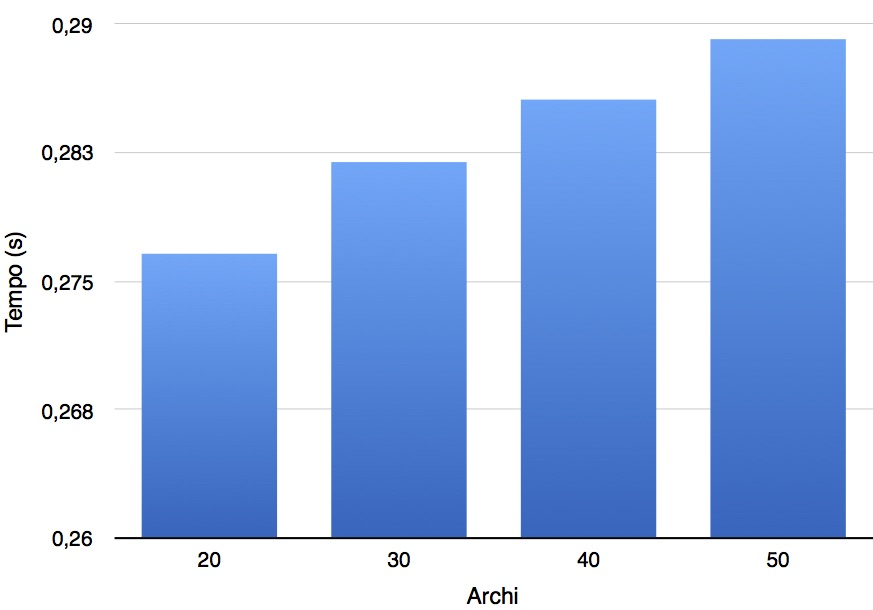
\includegraphics[scale=.25]{img/beta4/10_4.jpg}
		\caption{Algoritmo Partition2}
	\end{minipage}\hfill
	% <-- needed to keep the imgs side by side
	\begin{minipage}{0.40\textwidth}
		\centering
		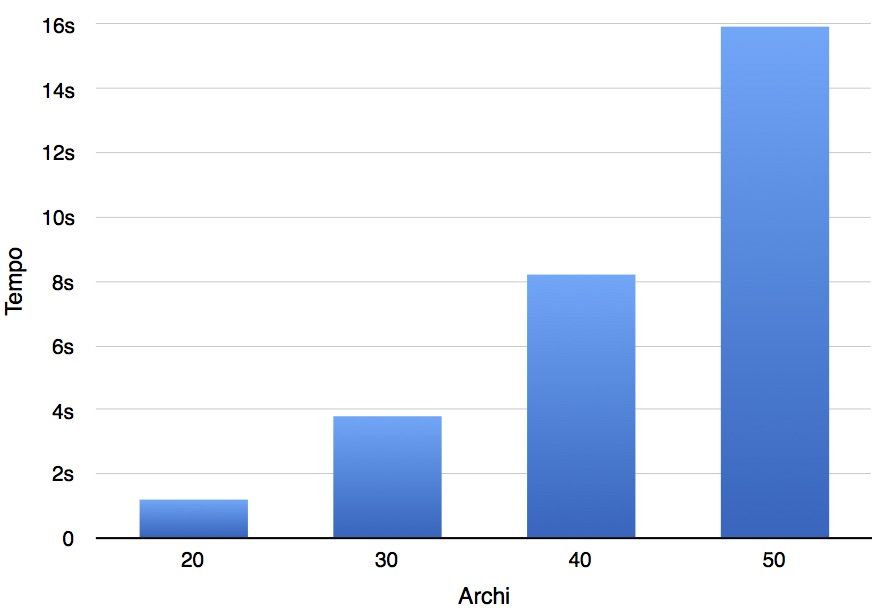
\includegraphics[scale=.25]{img/iole_beta4/iole_10_4.jpg}
		\caption{Algoritmo Partition}
	\end{minipage}
	\caption*{\textit{n = 10}}
\end{figure}
\begin{figure}[h!]
	\vspace*{1cm}
	\begin{minipage}{0.40\textwidth}
		\centering
		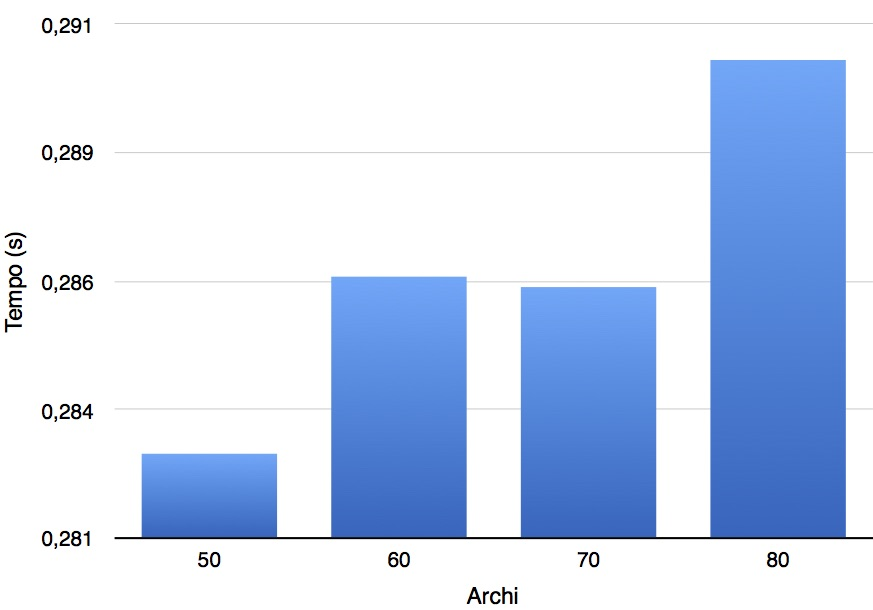
\includegraphics[scale=.25]{img/beta4/15_4.jpg}
		\caption{Algoritmo Partition2}
	\end{minipage}\hfill
	% <-- needed to keep the imgs side by side
	\begin{minipage}{0.40\textwidth}
		\centering
		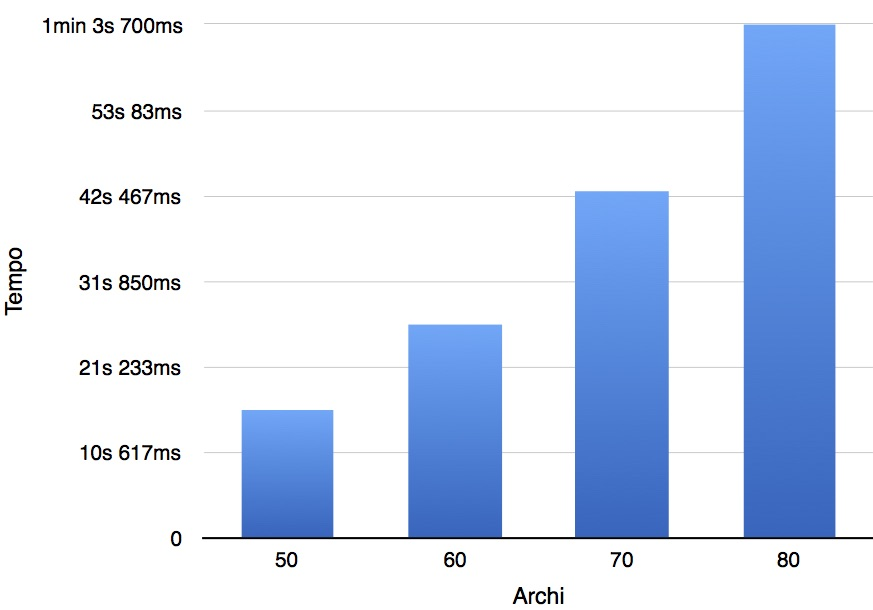
\includegraphics[scale=.25]{img/iole_beta4/iole_15_4.jpg}
		\caption{Algoritmo Partition}
	\end{minipage}
	\caption*{\textit{n = 15}}
\end{figure}
\begin{figure}[h!]
	\vspace*{1cm}
	\begin{minipage}{0.40\textwidth}
		\centering
		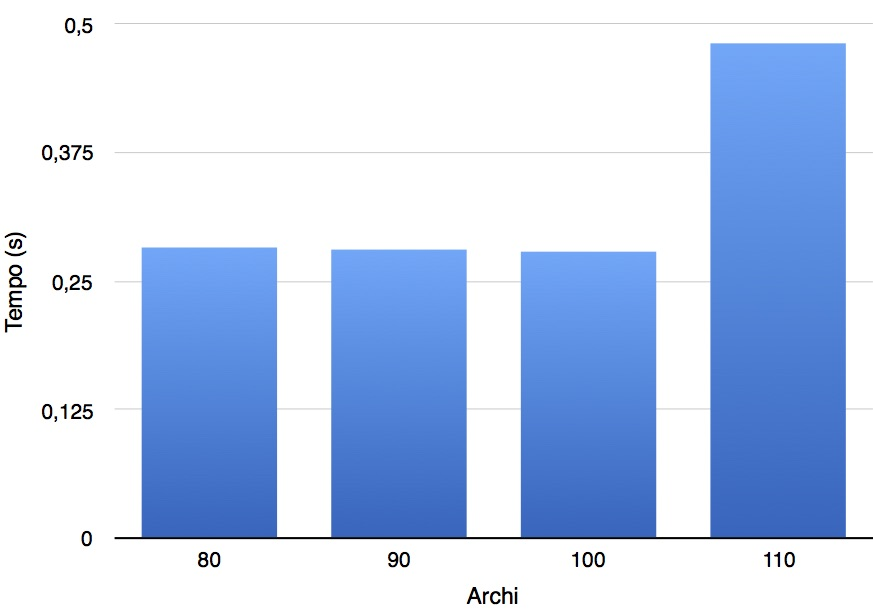
\includegraphics[scale=.25]{img/beta4/20_4.jpg}
		\caption{Algoritmo Partition2}
	\end{minipage}\hfill
	% <-- needed to keep the imgs side by side
	\begin{minipage}{0.40\textwidth}
		\centering
		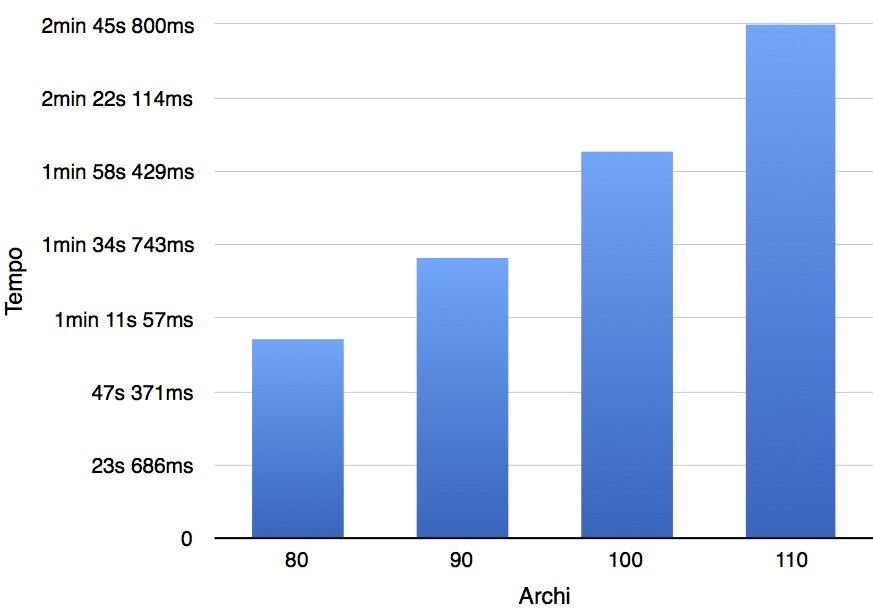
\includegraphics[scale=.25]{img/iole_beta4/iole_20_4.jpg}
		\caption{Algoritmo Partition}
	\end{minipage}
	\caption*{\textit{n = 20}}
\end{figure}
\begin{figure}[h!]
	\vspace*{1cm}
	\begin{minipage}{0.40\textwidth}
		\centering
		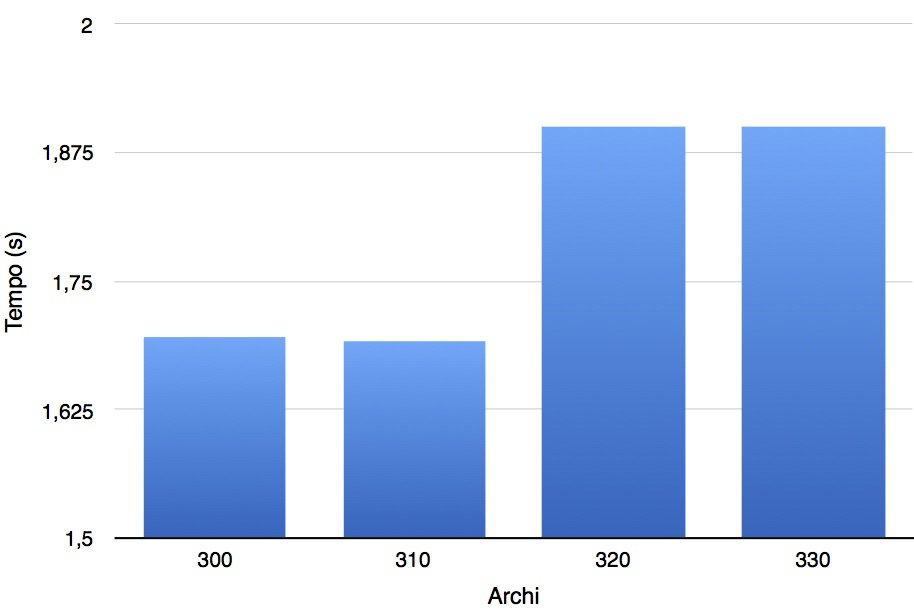
\includegraphics[scale=.25]{img/beta4/35_4.jpg}
		\caption{Algoritmo Partition2}
	\end{minipage}\hfill
	% <-- needed to keep the imgs side by side
	\begin{minipage}{0.40\textwidth}
		\centering
		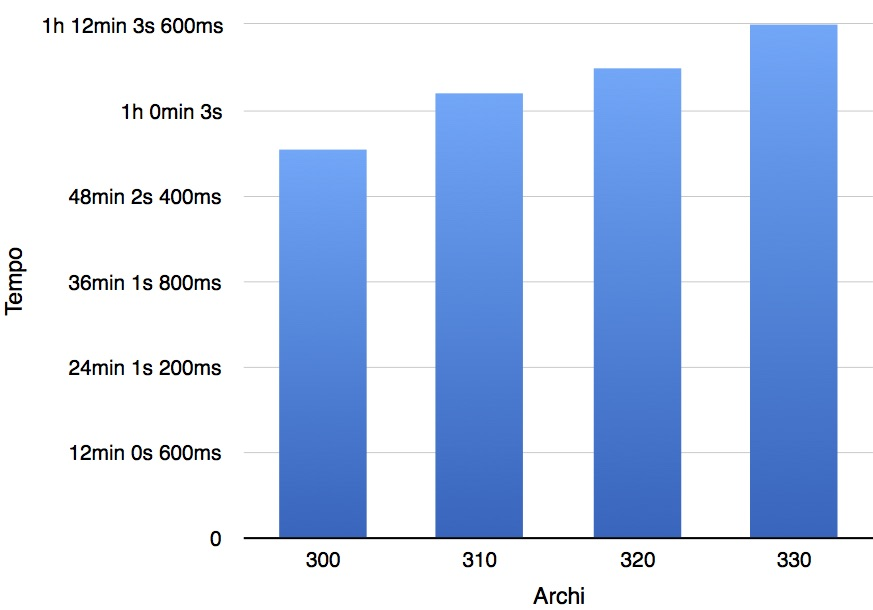
\includegraphics[scale=.25]{img/iole_beta4/iole_35_4.jpg}
		\caption{Algoritmo Partition}
	\end{minipage}
	\caption*{\textit{n = 35}}
\end{figure}
\begin{figure}[h!]
	\vspace*{1cm}
	\begin{minipage}{0.40\textwidth}
		\centering
		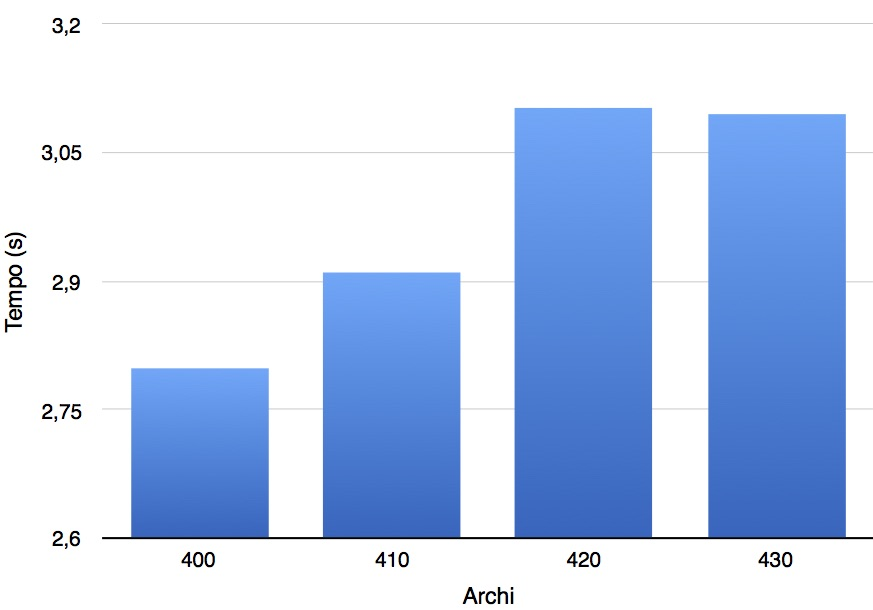
\includegraphics[scale=.25]{img/beta4/40_4.jpg}
		\caption{Algoritmo Partition2}
	\end{minipage}\hfill
	% <-- needed to keep the imgs side by side
	\begin{minipage}{0.40\textwidth}
		\centering
		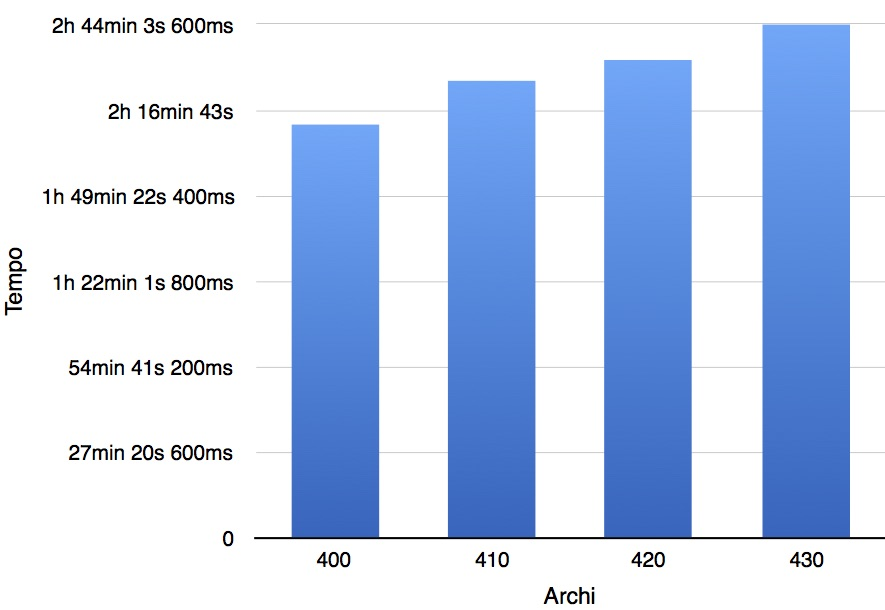
\includegraphics[scale=.25]{img/iole_beta4/iole_40_4.jpg}
		\caption{Algoritmo Partition}
	\end{minipage}
	\caption*{\textit{n = 40}}
\end{figure}
\begin{figure}[h!]
	\vspace*{1cm}
	\begin{minipage}{0.40\textwidth}
		\centering
		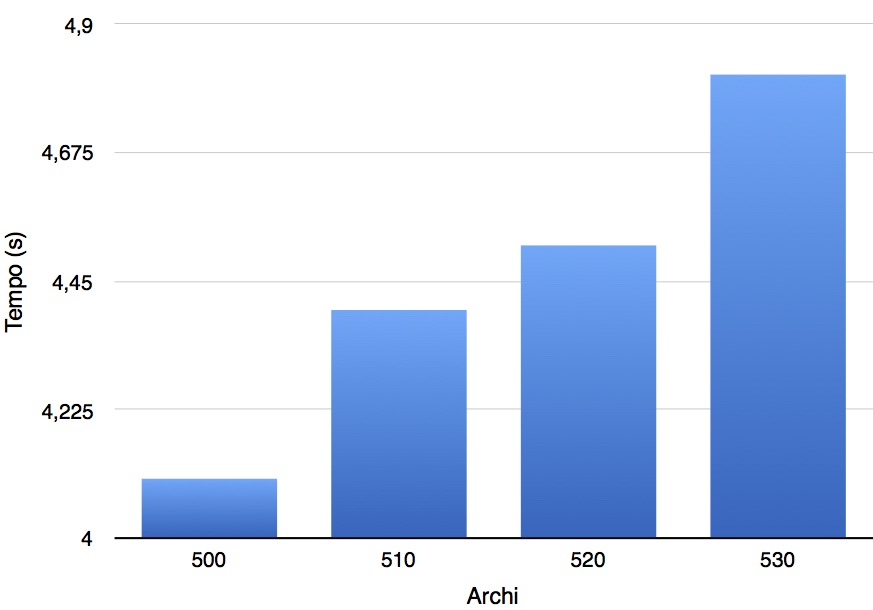
\includegraphics[scale=.25]{img/beta4/45_4.jpg}
		\caption{Algoritmo Partition2}
	\end{minipage}\hfill
	% <-- needed to keep the imgs side by side
	\begin{minipage}{0.40\textwidth}
		\centering
		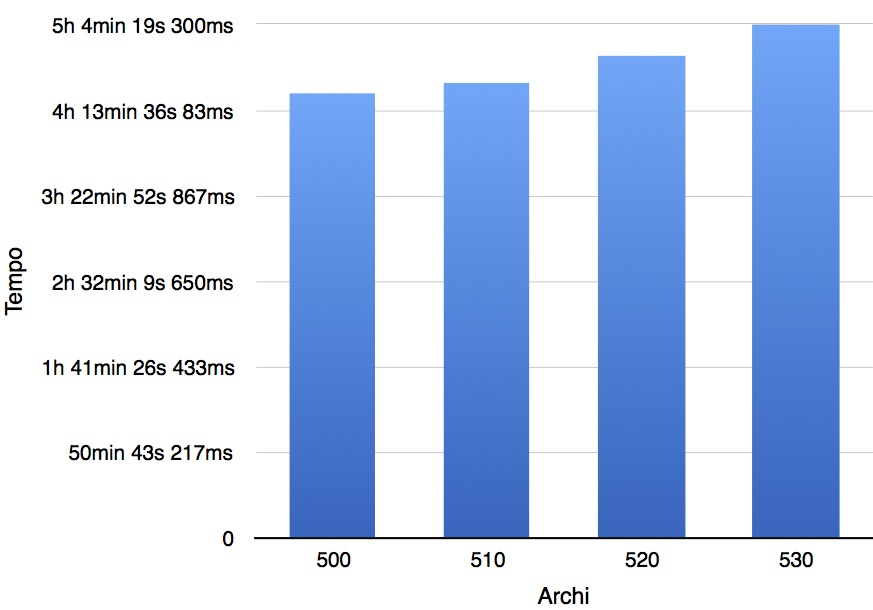
\includegraphics[scale=.25]{img/iole_beta4/iole_45_4.jpg}
		\caption{Algoritmo Partition}
	\end{minipage}
	\caption*{\textit{n = 45}}
\end{figure}
Come è possibile notare dai risultati, l'algoritmo Partition2 ha un netto margine di guadagno in termini di efficienza rispetto all'algoritmo Partition, il quale inizia a soffrire già con un grafo avente 20 nodi ed 90 archi, superando il minuto d'esecuzione contro i 250 ms della versione proposta da questo lavoro di tesi. Di seguito viene mostrato l'andamento del running time per l'algoritmo Partition2 al variare della taglia del grafo nel numero di nodi ed archi. 
\begin{figure}[h!]
	\vspace*{1cm}
	\centering
	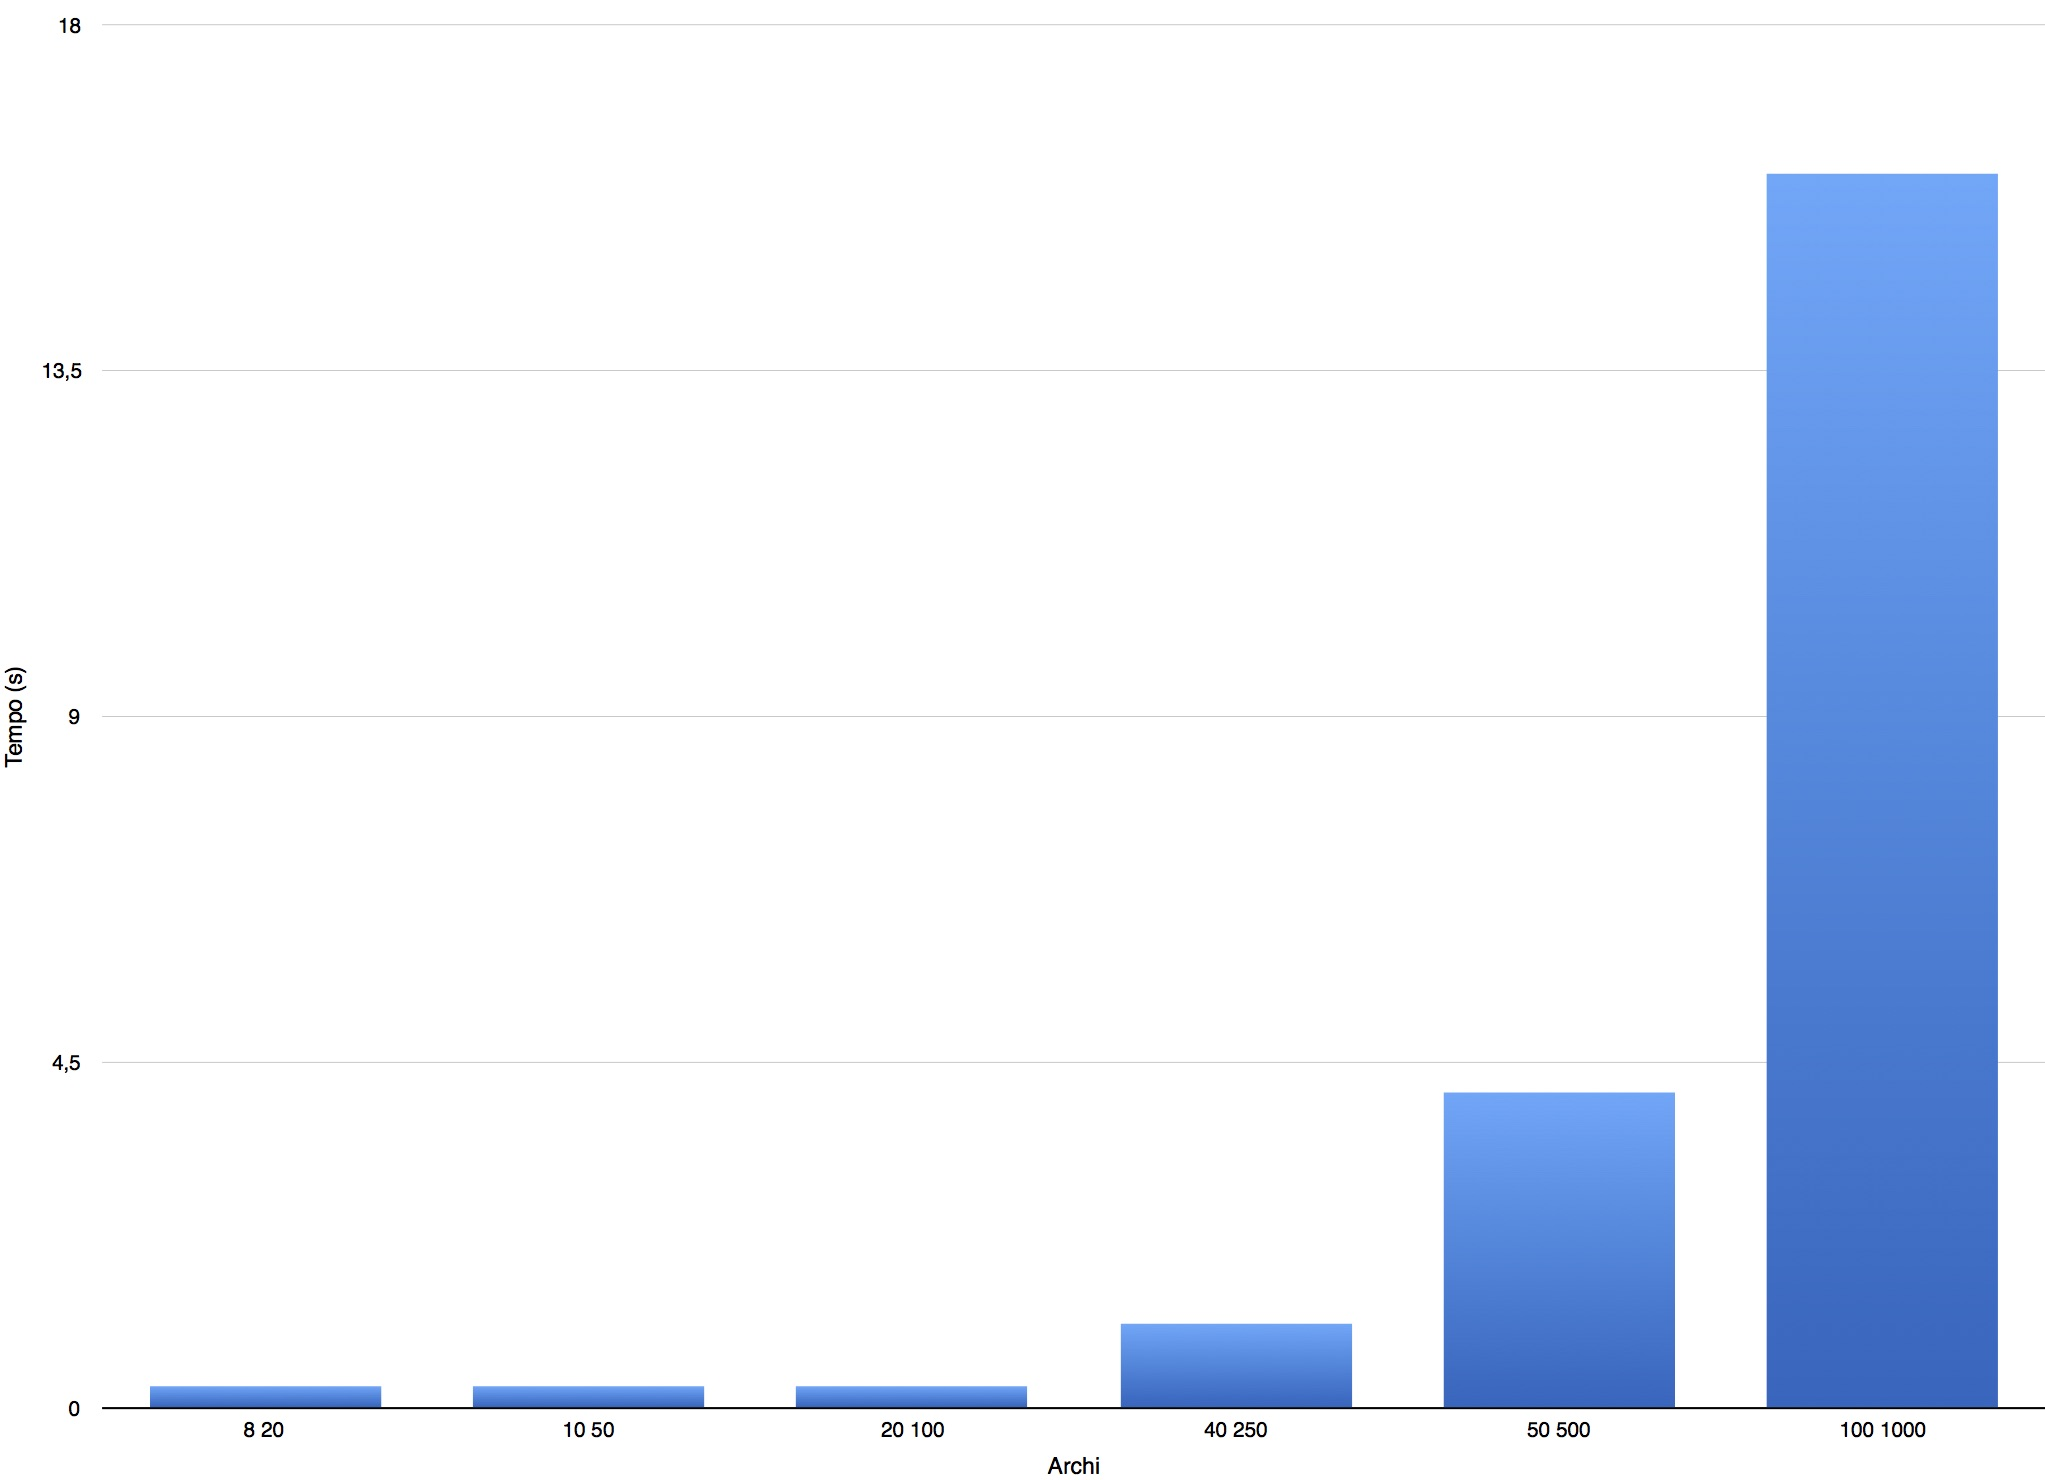
\includegraphics[scale=.15]{img/scala.jpg}
	\caption{Algoritmo Partition2 al variare di n ed m.}
\end{figure}
\begin{table}[]
	\centering
	\begin{tabular}{|c|c|c|c|c|c|c|c|}
		\hline
		n & m & B & $\beta$ & $\epsilon$ & s & t & Tempo (s)\\ \hline
		500 & 1000 & 20 & 0.4 & 0.1 & 1 & 2 & 399.465704\\ \hline
	\end{tabular}
	\caption{Algoritmo Partition2 \textit{n = 500, m = 5000}.}\label{tab:5000}
\end{table}
L'esecuzione riportata in Tabella \ref{tab:5000} è stata tenuta fuori dal precedente grafico per motivi di scala: è possibile apprezzare l'efficienza dell'algoritmo Partition2 anche in questo caso, in quanto impiega circa 400 secondi per calcolare la funzione di partizione su un grafo con 500 nodi e 5000 archi, che già si avvicina ad un'istanza del mondo reale.\\
Grazie ai miglioramenti ottenuti, si è scelto di eseguire anche un test su grafi di dimensioni maggiori, sempre al variare dei parametri $n$ ed $m$, mantenendo i parametri $B = 20, \beta = 0.4, \epsilon = 0.1$ invariati.
\begin{figure}[h!]
	\vspace*{1cm}
	\begin{minipage}{0.40\textwidth}
		\centering
		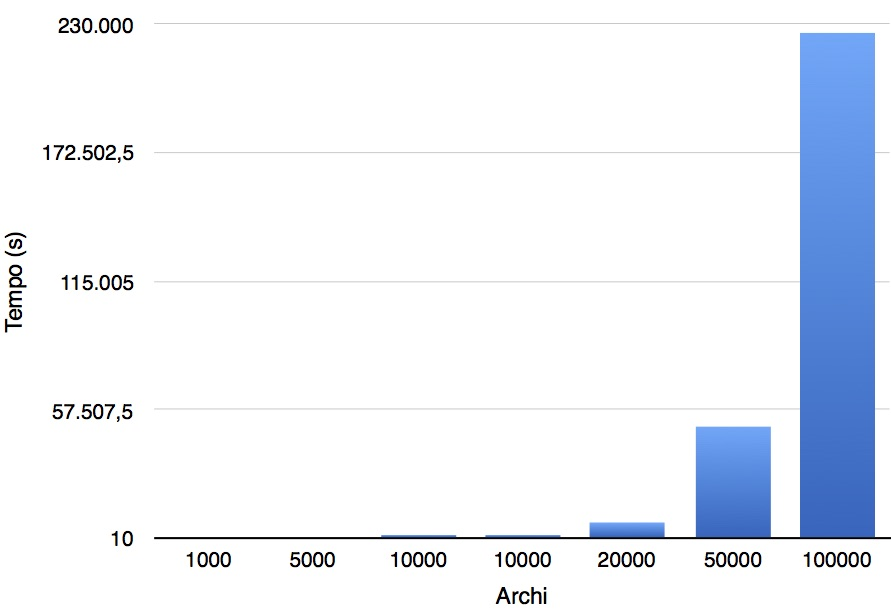
\includegraphics[scale=.25]{img/big.jpg}
		\caption{Scala lineare}
	\end{minipage}\hfill
	% <-- needed to keep the imgs side by side
	\begin{minipage}{0.40\textwidth}
		\centering
		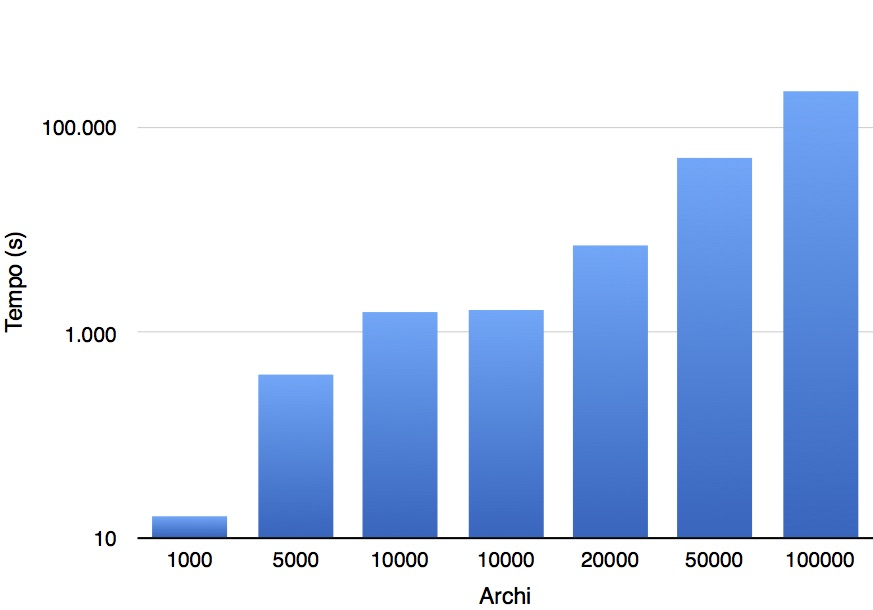
\includegraphics[scale=.25]{img/big_log.jpg}
		\caption{Scala logaritmica}
	\end{minipage}
	\caption*{Grafi di dimensioni maggiori.}
\end{figure}
\clearpage
\subsection{Parametro $\epsilon$}
I seguenti grafici riportano i risultati ottenuti nei test di accuratezza. Il parametro $\epsilon$ è stato fatto variare da $10^{-1}$ a $10^{-4}$.\\
È possibile notare come il tempo aumenti notevolmente nel passaggio da $\epsilon = 10^{-3}$ a $\epsilon = 10^{-4}$, ma sia comunque accettabile anche considerando il fatto che l'algoritmo Partition non è in grado di ottenere tempi ragionevoli già a partire da $\epsilon$ minore di $10^{-1}$.
\begin{figure}[!htb]
	\vspace*{1cm}
	\centering
	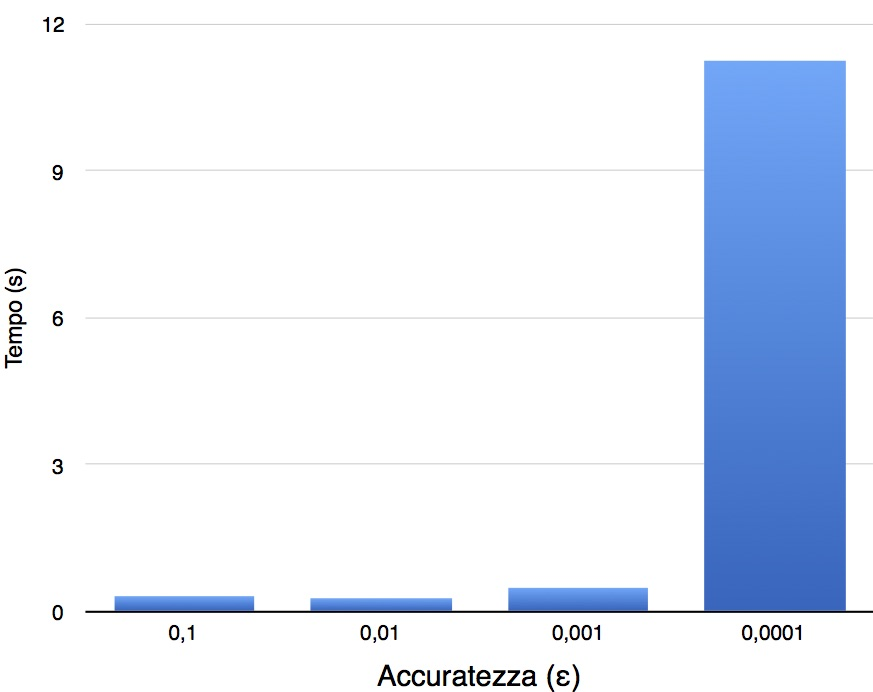
\includegraphics[scale=.3]{img/eps/8.jpg}
	\caption{Algoritmo Partition2 $n = 8, m = 20$.}
\end{figure}
\begin{figure}[!htb]
	\vspace*{1cm}
	\centering
	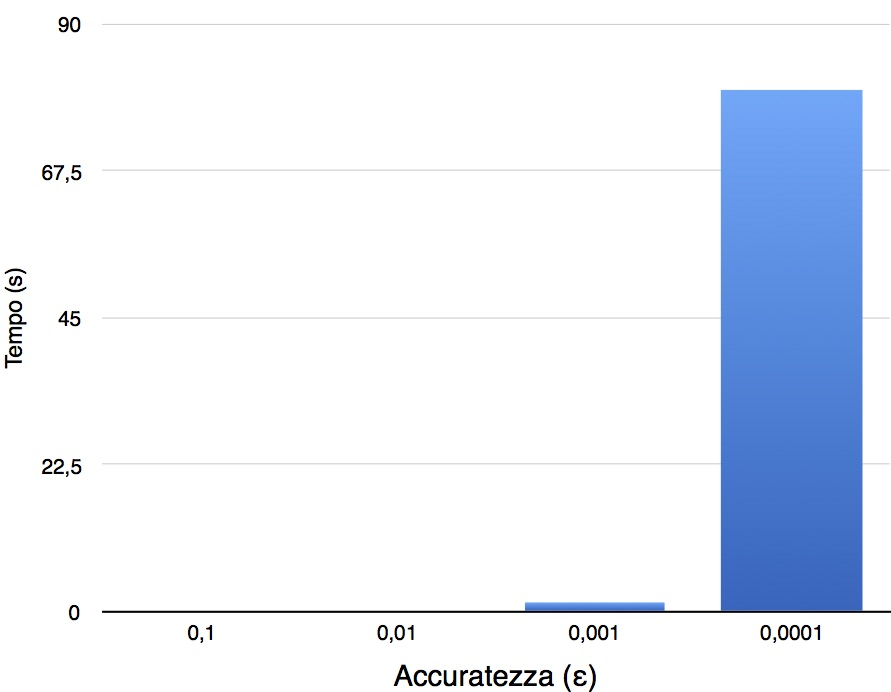
\includegraphics[scale=.3]{img/eps/10.jpg}
	\caption{Algoritmo Partition2 $n = 10, m = 50$.}
\end{figure}
\begin{figure}[!htb]
	\vspace*{1cm}
	\centering
	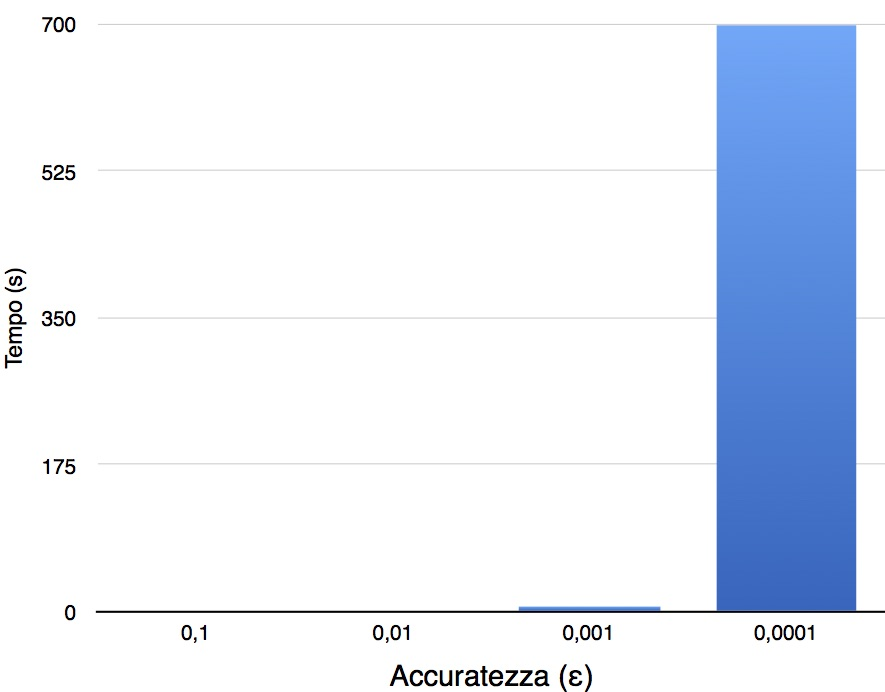
\includegraphics[scale=.3]{img/eps/20.jpg}
	\caption{Algoritmo Partition2 $n = 20, m = 100$.}
\end{figure}
\begin{figure}[!htb]
	\vspace*{1cm}
	\centering
	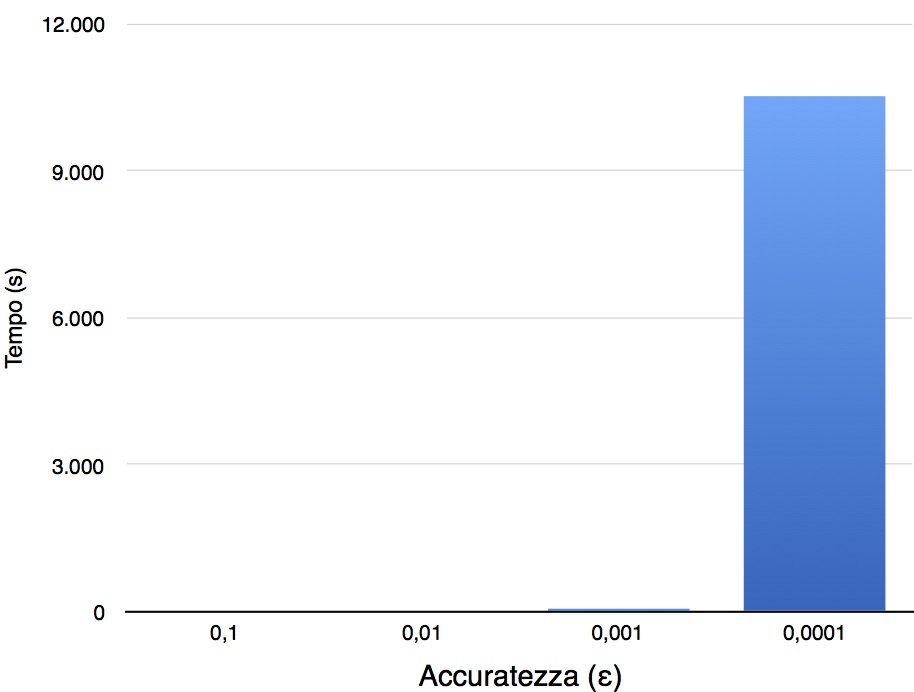
\includegraphics[scale=.3]{img/eps/40.jpg}
	\caption{Algoritmo Partition2 $n = 40, m = 250$.}
\end{figure}
\begin{figure}[!htb]
	\vspace*{1cm}
	\centering
	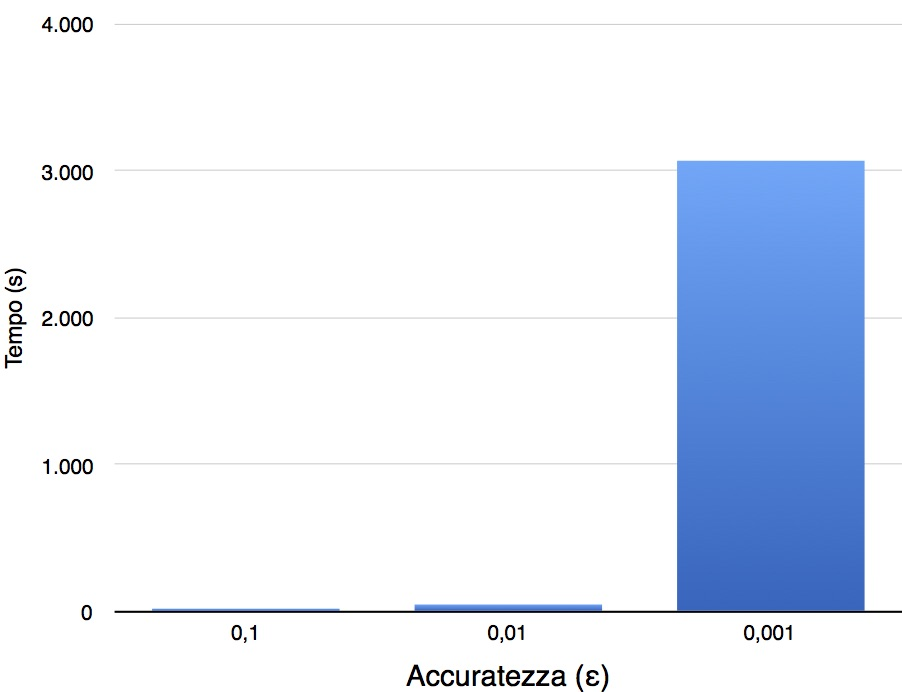
\includegraphics[scale=.3]{img/eps/100.jpg}
	\caption{Algoritmo Partition2 $n = 100, m = 1000$.}
\end{figure}
\clearpage
\subsection{Parametro $\mu$}
I grafici presenti in questa sezione rappresentano l'andamento dell'algoritmo Partition2 al variare dei valori $B$ e $\beta$. Come si ricorda in \ref{mu}, da tali valori dipende $\mu$ e di conseguenza sulla complessità del generatore atto a simulare la catena di Markov, per il Teorema \ref{thm:gen}. Il valore di $B$ è stato fatto variare da 20 ad 8 in tutti i test seguenti, modificando di conseguenza $\beta$ (parametro di razionalità) per mantenere $\mu$ in un range tra 1 e 0.75, come mostrato in Tabella \ref{tab:bbetamu}.
\begin{table}[]
	\centering
	\begin{tabular}{|c|c|c|}
		\hline
		B  & $\beta$  & $\mu$               \\ \hline
		20 & 0.4      & 0.99999977492967584 \\ \hline
		15 & 0.122119 & 0.95000040724956369 \\ \hline
		10 & 0.147222 & 0.90000009697914363 \\ \hline
		12 & 0.104679 & 0.84999866466785234 \\ \hline
		10 & 0.109861 & 0.799999176077972   \\ \hline
		8  & 0.121619 & 0.74999865489104856 \\ \hline
	\end{tabular}
	\caption{Parametri utilizzati.}
	\label{tab:bbetamu}
\end{table}
\begin{figure}[h!]
	\vspace*{1cm}
	\centering
	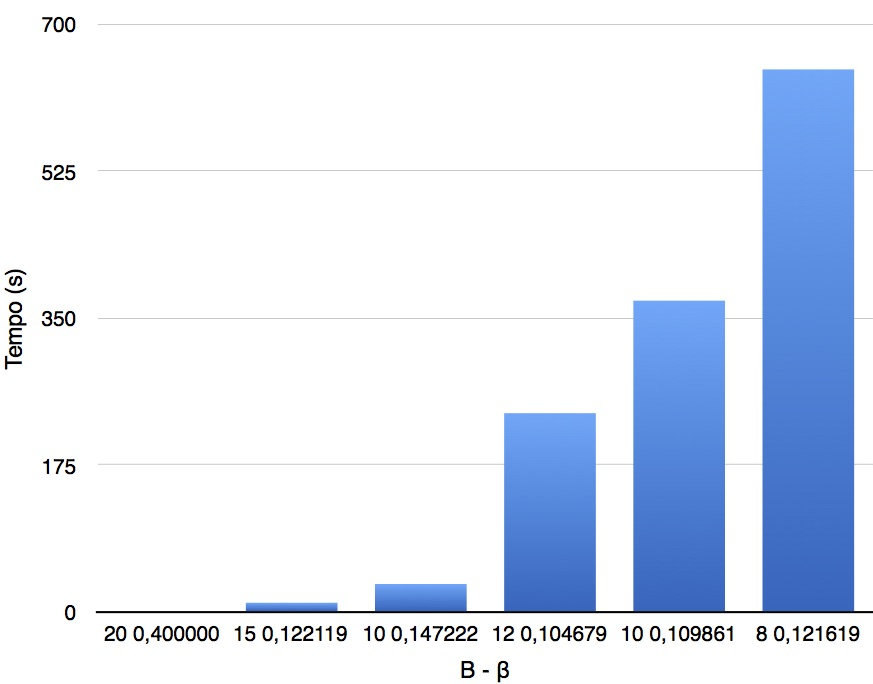
\includegraphics[scale=.3]{img/Bbeta/8_20.jpg}
	\caption{Algoritmo Partition2 $n = 8, m = 20$.}
\end{figure}
\begin{figure}[h!]
	\vspace*{1cm}
	\centering
	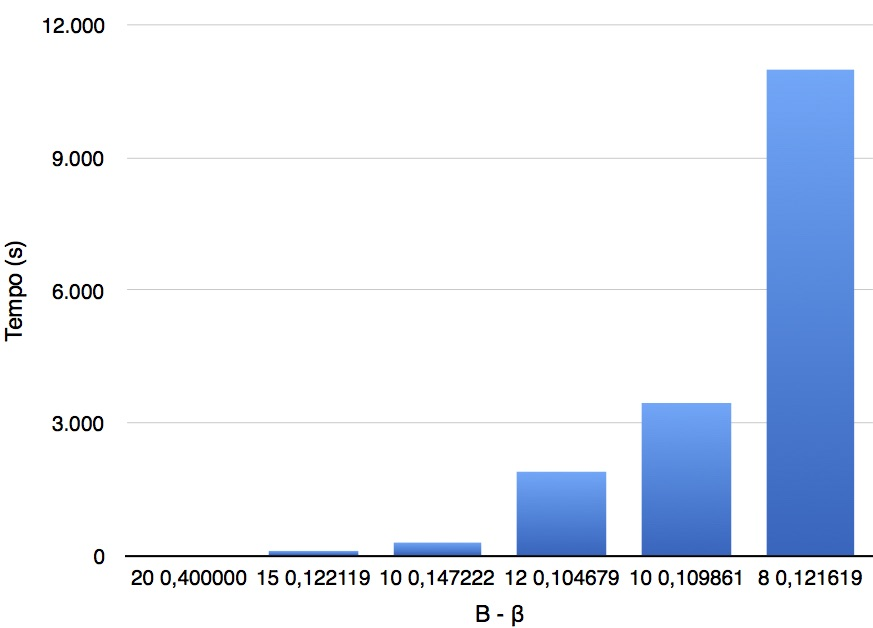
\includegraphics[scale=.3]{img/Bbeta/10_50.jpg}
	\caption{Algoritmo Partition2 $n = 10, m = 50$.}
\end{figure}
\begin{figure}[h!]
	\vspace*{1cm}
	\centering
	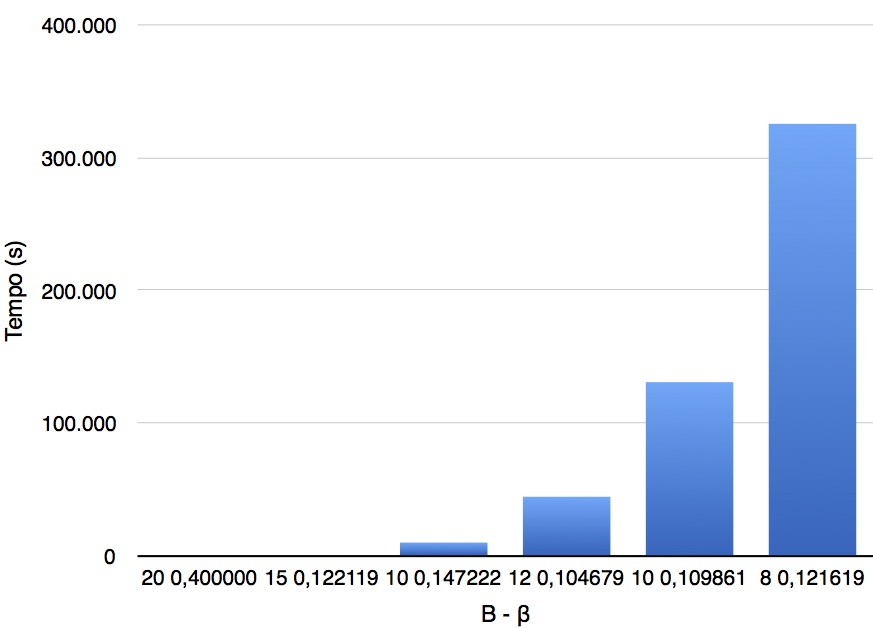
\includegraphics[scale=.3]{img/Bbeta/20_100.jpg}
	\caption{Algoritmo Partition2 $n = 20, m = 100$.}
\end{figure}
\begin{figure}[h!]
	\vspace*{1cm}
	\centering
	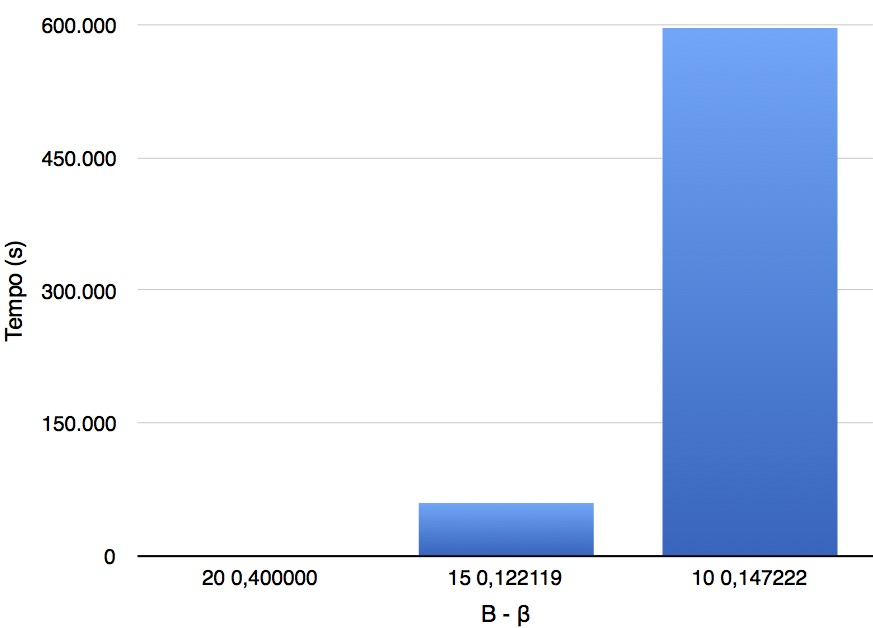
\includegraphics[scale=.3]{img/Bbeta/40_250.jpg}
	\caption{Algoritmo Partition2 $n = 40, m = 250$.}
\end{figure}
È possibile notare dai risultati ottenuti come, al decrescere di $\mu$ il tempo cresca piuttosto linearmente, confermando quanto indicato dal Teorema \ref{thm:gen}.
\clearpage



\section{The Effectiveness of Advertising}
Questa sezione presenta un esempio di applicazione dell'algoritmo sviluppato: la simulazione di una campagna pubblicitaria. si hanno due prodotti da promuovere e si è interessati a calcolare la \textit{magnetizzazione} del sistema, ovvero il numero atteso di persone che sceglieranno di utilizzare un prodotto piuttosto che l'altro. Per raggiungere tale scopo è necessario sfruttare il lavoro proposto nel Capitolo \ref{chap6} riguardante il \textit{mean magnetic moment}.
\subsection{Scenario}
Si consideri una \textit{network} $G = (V,E)$ con $|V| = n$, in cui ogni vertice rappresenta un giocatore (agente) avente a disposizione due possibili scelte, cioè i due prodotti, detti anche \textit{strategie}, denotati da 0 e 1.\\
Ad ogni agente della rete è assegnato un \textit{profilo} $x = (x_1, \cdots, x_n) \in \Omega = {0, 1}^n$. Ad ogni arco $e = (u, v) \in E$ è associato un \textit{two-player game} con funzione potenziale 
\begin{equation}
\Phi_e(x) = 
\begin{cases}
-a, & \text{se}\ x_u = x_v = 1;\\
-b, & \text{se}\ x_u = x_v = 0;\\
0, & \text{altrimenti}
\end{cases}
\label{potentfun}
\end{equation}
con $a, b \geq 0$. Si assume che ogni agente preferisca coordinarsi con i suoi vicini piuttosto che giocare una strategia differente.\\
Si consideri ora la situazione in cui ogni agente debba scegliere una strategia e giocare tale strategia in ogni gioco in cui esso è coinvolto, cioè su ogni arco adiacente. Questa situazione modella un gioco con funzione potenziale
\begin{equation*}
	\Phi(x) = \sum_{e\in E}{\Phi_e(x)}.
	\label{eqpotfun}
\end{equation*}
È noto che la \textit{Logit Dynamics} per questo tipo di gioco converge alla distribuzione
\begin{equation*}
	\pi(x) = \frac{e^{\beta\Phi(x)}}{Z},
	\label{logitdistr}
\end{equation*}
dove Z è il fattore di normalizzazione e $\beta$ rappresenta il livello di razionalità.\\
Tenendo a mente la definizione di \textit{mean magnetic moment} fornita in \ref{mmm}
\begin{equation*}
\mathcal{M} = \beta^{-1}\partial(lnZ)/\partial\beta,
\end{equation*}
il Teorema \ref{thm:fpras_mmm} che afferma
\textit{ ``Esiste un fpras per il mean magnetic moment $\mathcal{M} = \beta^{-1}\partial(lnZ)/\partial\beta$, dove $Z$ è la partition function di un sistema di Ising ferromagnetico.''}

Sono stati apportati notevoli miglioramenti al metodo di approssimazione della funzione \textit{odd(X)}, come mostrato in \ref{ssec:betteroddx}, che hanno portato alla realizzazione degli algoritmi presentati in \ref{ssec:algooddx}.\\
La simulazione è stata realizzando avvalendosi dell'algoritmo \ref{alg:eoddx}, il quale a sua volta fa uso di \ref{alg:est_f_threshold}. Sono stati scelti i parametri che hanno fornito i migliori risultati nei tempi d'esecuzione degli esperimenti precedenti, cioè $B = 20, \beta = 0.4$ ed $\epsilon = 0.1$.
Il grafico seguente riporta i tempi di alcune esecuzioni, al variare del grafo di input.
\begin{figure}[h!]
	\vspace*{1cm}
	\centering
	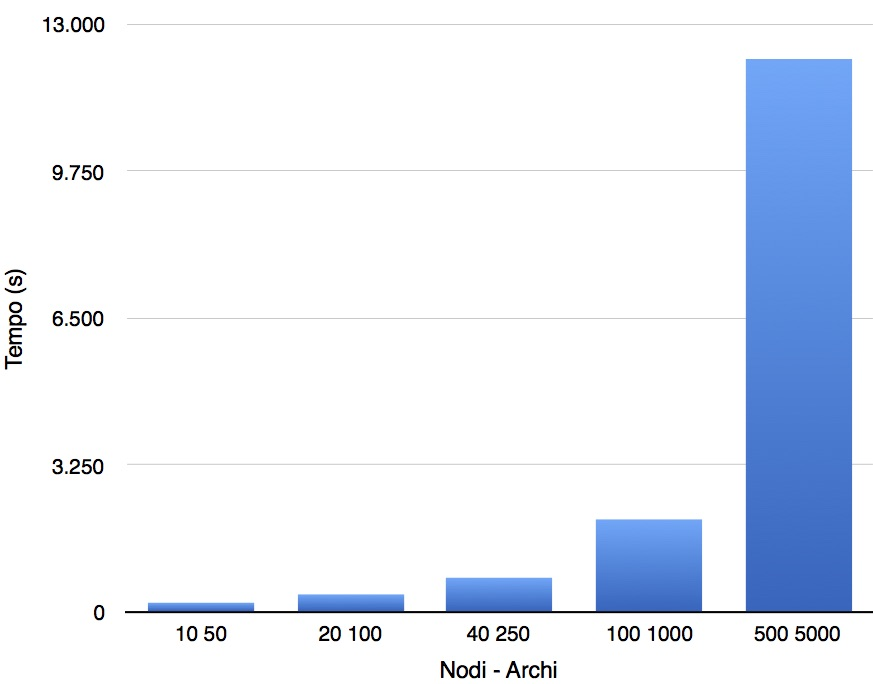
\includegraphics[scale=.3]{img/mmm.jpg}
	\caption{Algoritmo Partition2 $n = 40, m = 250$.}
\end{figure}
La Tabella \ref{tab:mmm} fornisce maggiori informazioni riguardo i dettagli di esecuzione dei test.
\begin{table}[]
	\centering
	\begin{tabular}{|c|c|c|c|c|c|c|c|}
		\hline
		nodi & archi & s & t & Tempo\\ \hline
		10& 50& 5950& 2& 3min 48s\\ \hline
		20& 100& 13218& 2& 6min 31s\\ \hline
		40& 250& 27754& 2& 12min 46s\\ \hline
		100& 1000& 71361& 2& 34min 15s\\ \hline
		500& 5000& 362075& 2& 3h 24min 17s\\ \hline
	\end{tabular}
	\caption{Simulazioni \textit{mean magnetic moment}.}\label{tab:mmm}
\end{table}
Il lavoro \cite{rinaldi2016approximation} riporta nel Capitolo 6 i risultati del test effettuato per un simile scenario e la Tabella \ref{tab:mmmrin} mostra il tempo impiegato per eseguire un test su un grafo con 10 nodi e 50 archi.
\begin{table}[]
	\centering
	\begin{tabular}{|c|c|c|c|c|c|c|c|}
		\hline
		nodi & archi & s & t & Tempo\\ \hline
		10& 50& 62245& 2& 14h 20m 16s\\ \hline
	\end{tabular}
	\caption{Simulazioni \textit{mean magnetic moment}.}\label{tab:mmmrin}
\end{table}
È evidente che tale implementazione sia impraticabile in situazioni reali, e allo stesso tempo è possibile apprezzare l'efficienza del lavoro proposto, che porta a termine lo stesso esperimento in circa 4 minuti rispetto alle 14 ore impiegate in precedenza. Inoltre, l'algoritmo che calcola il \textit{mean magnetic moment} presentato in questa tesi presenta tempi ragionevoli anche su istanza di dimensioni discrete, come nel caso del grafo a 500 nodi e 5000 archi su cui impiega circa 3 ore e 30 minuti per calcolarne la magnetizzazione.
\clearpage
\section{Test su dati reali}
Il lavoro svolto ha reso possibile l'obiettivo preposto: testare l'algoritmo \textbf{Partition2} su dataset provenienti dal mondo reale.\\
\subsection{Dataset Gnutella}
Il dataset utilizzato è una delle network messe a disposizione dallo \textit{Stanford Network Analysis Project} (SNAP) \cite{snapnets} e rappresenta una sequenza di 9 \textit{snapshots} della rete di condivisione file \textit{peer-to-peer} Gnutella a partire da Agosto 2002. I nodi rappresentano gli \textit{host} nella topologia della rete Gnutella e gli archi rappresentano le connessioni tra di essi. In Tabella \ref{tab:gnutella} vengono riportate informazioni dettagliate sul dataset.
\begin{table}[h!]
	\centering
	\begin{tabular}{|c|c|}
		\hline
		Nodi& 6301\\ \hline
		Archi& 20777\\ \hline
		Nodi nella più grande WCC& 6299 (1.000)\\ \hline
		Archi nella più grande WCC& 20776 (1.000)\\ \hline
		Nodi nella più grande SCC& 2068 (0.328)\\ \hline
		Archi nella più grande SCC& 9313 (0.448)\\ \hline
		Coefficiente di average clustering& 0.0109\\ \hline
		Numero di triangoli& 2383\\ \hline
		Frazione di triangoli chiusi& 0.006983\\ \hline
		Diametro (\textit{shortest path} più lungo)& 9\\ \hline
	\end{tabular}
	\caption{Statistiche del grafo Gnutella (SNAP).}\label{tab:gnutella}
\end{table}

L'algoritmo \textbf{Partition2} ha terminato la sua esecuzione in 59.129,02 secondi, cioè in circa 16 ore e 42 minuti.
\subsection{Dataset Facebook}
Il dataset utilizzato in quest'ultimo esperimento è anch'esso messo a disposizione dallo \textit{Stanford Network Analysis Project} (SNAP) \cite{snapnets} e rappresenta uno \textit{snapshot} di un sottografo della rete di amicizie di Facebook. Gli utenti sono rappresentati dai nodi e le relazioni di amicizia sono rappresentate dagli archi. Il grafo in questione è una vera e propria rete sociale e presenta tutte le caratteristiche tipiche di questo tipo di reti, come l'alto numero di triangoli ed un discreto coefficiente di \textit{average clustering}. La Tabella \ref{tab:facebook} mostra ulteriori informazioni sul dataset.\\
\begin{table}[h!]
	\centering
	\begin{tabular}{|c|c|}
		\hline
		Nodi& 4039\\ \hline
		Archi& 88234\\ \hline
		Nodi nella più grande WCC& 4039 (1.000)\\ \hline
		Archi nella più grande WCC& 88234 (1.000)\\ \hline
		Nodi nella più grande SCC& 4039 (1.000)\\ \hline
		Archi nella più grande SCC& 88234 (1.000)\\ \hline
		Coefficiente di average clustering& 0.6055\\ \hline
		Numero di triangoli& 1612010\\ \hline
		Frazione di triangoli chiusi& 0.2647\\ \hline
		Diametro (\textit{shortest path} più lungo)& 8\\ \hline
	\end{tabular}
	\caption{Statistiche del grafo Facebook (SNAP).}\label{tab:facebook}
\end{table}
L'algoritmo \textbf{Partition2} ha terminato la sua esecuzione in 684.060,44 secondi, cioè circa 7 giorni. Considerando le caratteristiche della rete, il tempo impiegato non è eccessivo.\\
Questo prova l'effettiva possibilità di poter essere utilizzato su reti del mondo reale.
\clearpage